\vspace{-0.2cm}
Learning manipulable representations of the world and its dynamics is central to AI. Joint-Embedding Predictive Architectures (JEPAs) offer a promising blueprint, but lack of practical guidance and theory has led to ad‑hoc R\&D. We present a comprehensive theory of JEPAs and instantiate it in {\bf LeJEPA}, a lean, scalable, and theoretically grounded training objective. First, we identify the isotropic Gaussian as the optimal distribution that JEPAs' embeddings should follow to minimize downstream prediction risk. Second, we introduce a novel objective--{\bf Sketched Isotropic Gaussian Regularization} (SIGReg)--to constrain embeddings to reach that ideal distribution. Combining the JEPA predictive loss with SIGReg yields LeJEPA with numerous theoretical and practical benefits: (i) single trade‑off hyperparameter, (ii) linear time and memory complexity, (iii) stability across hyper-parameters, architectures (ResNets, ViTs, ConvNets) and domains,  (iv) heuristics-free, e.g., no stop‑gradient, no teacher–student, no hyper-parameter schedulers, and (v) distributed training-friendly implementation requiring only $\approx$50 lines of code. Our empirical validation covers 10+ datasets, 60+ architectures, all with varying scales and domains. As an example, using imagenet-1k for pretraining and linear evaluation with frozen backbone, LeJEPA reaches 79\% with a ViT-H/14. We hope that the simplicity and theory-friendly ecosystem offered by LeJEPA will reestablish self-supervised pre-training as a core pillar of AI research (\href{https://github.com/rbalestr-lab/lejepa}{GitHub repo}).
\\[0em]
\begin{center}

    \vspace{-0.7cm}
    % Top row
    \begin{minipage}{0.44\linewidth}
        \centering
        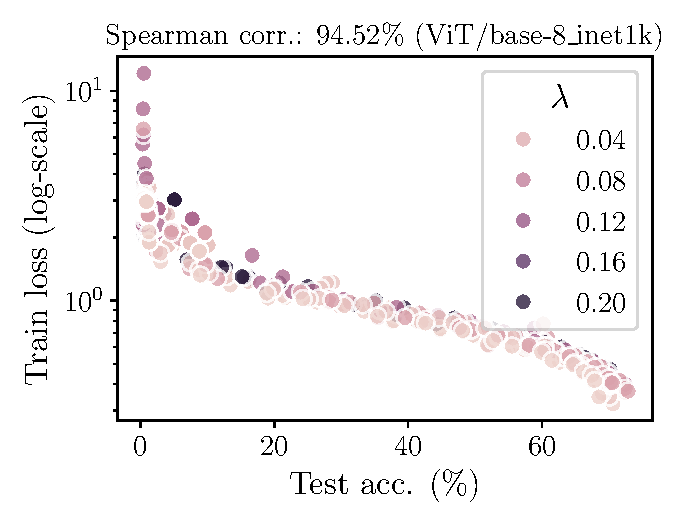
\includegraphics[width=\linewidth]{toy_figures/exps/loss_corr/loss_corr_ViT-base-8_inet1k.pdf}
    \end{minipage}%
    \hfill
    \begin{minipage}{0.54\linewidth}
        \centering
        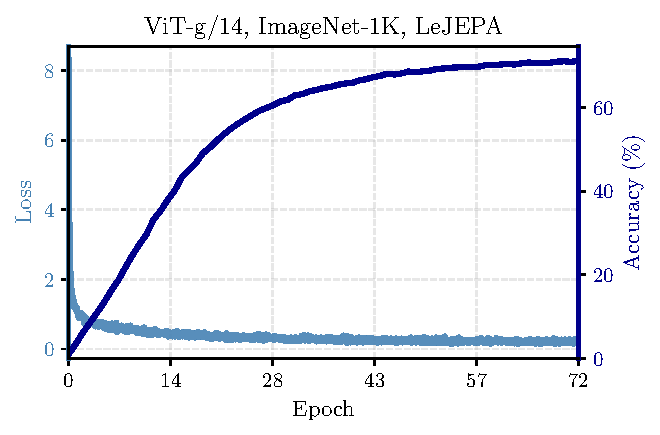
\includegraphics[width=\linewidth]{toy_figures/teaser/training_comparison.pdf}
    \end{minipage}
    
    \vspace{0.03cm}
    
    % Bottom row
    \begin{minipage}{0.44\linewidth}
        \centering
        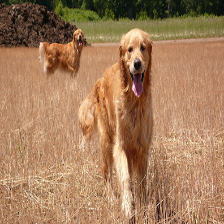
\includegraphics[width=0.485\linewidth]{toy_figures/pca/n02099601_5984_original.png}\hfill
        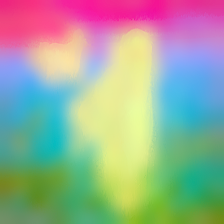
\includegraphics[width=0.485\linewidth]{toy_figures/pca/n02099601_5984_pca.png}
    \end{minipage}%
    \hfill
    \begin{minipage}{0.54\linewidth}
        \centering
        \footnotesize
        \setlength{\tabcolsep}{2.5pt}
        \renewcommand{\arraystretch}{0.95}
        \begin{tabular}{lcccc}
        \toprule
         & \multicolumn{2}{c}{\textbf{Full FT}} & \multicolumn{2}{c}{\textbf{Frozen}} \\
        \cmidrule(lr){2-3} \cmidrule(lr){4-5}
        \textbf{Method} & \textbf{1-sh} & \textbf{Full} & \textbf{1-sh} & \textbf{Full} \\
        \midrule
        \multicolumn{5}{l}{\textit{LeJEPA (in-domain)}} \\
        \;\;ConvNeXt-V2 Nano & \textbf{29.42} & 82.72 & 28.74 & 76.52 \\
        \;\;ResNet-34 & 24.27 & \textbf{83.28} & \textbf{31.08} & \textbf{78.17} \\
        \midrule
        \multicolumn{5}{l}{\textit{Frontier (transfer)}} \\
        \;\;DINOv2 ViT-S/16 & 21.05 & 78.34 & 27.68 & 67.62 \\
        \;\;DINOv3 ViT-S/16 & 24.71 & 81.60 & 30.17 & 71.38 \\
        \bottomrule
        \end{tabular}
    \end{minipage}
    
    \vspace{0.05cm}
    \captionof{figure}{\textbf{LeJEPA overview.} \textbf{Top-left:} Training loss exhibits strong correlation with downstream linear probe performance on ImageNet-1k (ViT-base), providing the first practical loss for model selection without supervised probing. \textbf{Top-right:} Training stability without heuristics even on 1.8B ViT-g models, stable training loss. \textbf{Bottom-left:} PCA features from ImageNet-1k pretrained LeJEPA ViT-Large demonstrate clear semantic relationships. \textbf{Bottom-right:} Galaxy10 in-domain results showcasing LeJEPA's in-domain pretraining consistently outperforms state-of-the-art frontier foundation models transfer learning (DINOv2/v3 trained on natural images) across data regimes from 1-shot to full supervision. This demonstrates that \textit{domain-specific SSL beats generic transfer learning}, even against massive-scale frontier models, when the framework scales effortlessly to any domain, model, and data scale.}
    \label{fig:teaser}
    \vspace{-0.5cm}
\end{center}